\documentclass{slide}
% \usepackage{pgfpages}

% \setbeameroption{show notes on second screen}

\title{Microkernel Architecture}
\subtitle{CSSE6400}
\author{Richard Thomas}
\date{\week{3}}

\usepackage{tabto}

\begin{document}

\maketitle

\point[So far\dots]{%
\begin{description}
    \item[Simplicity] -- Monolith, Pipeline
    \item[Modularlity] -- Layered, Pipeline
\end{description}}
\note{Emphasise quality attributes and how architectural styles deliver those attributes.}

\definition{Extensibility}{Features or extensions can be easily added to the software over its lifespan.}

\questionanswer{How easy is it to extend \highlight{Monolith}, \highlight{Layered} or \highlight{Pipeline}?}
{\begin{description}
    \item<2->[Monolith] -- Everything in one container \tabto{15em}
\includegraphics[trim=22 19 22 15,clip,width=10mm]{../../shared/images/thumbs-down.png}
    \item<3->[Layered] -- Typically all layers \tabto{15em}
\includegraphics[trim=22 19 22 15,clip,width=10mm]{../../shared/images/thumbs-down.png}
    \item<4->[Pipeline] -- Create a new filter \tabto{15em}
\includegraphics[width=10mm]{../../shared/images/thumbs-up.png}
\end{description}}
\note{Discuss issues of extending a monolith or layered architecture.}

\definition{Interoperability}{Software can easily share information and exchange data with internal components and other systems.}

\questionanswer{What about interoperability?}
{\begin{description}
    \item<2->[Monolith] -- Everything in one container
    {\LARGE\begin{itemize}
        \setlength{\itemindent}{2em}
        \item Internal ~
\includegraphics[width=7.5mm]{../../shared/images/thumbs-up.png}
                 \tabto{9em}External ~
\includegraphics[trim=22 19 22 15,clip,width=7.5mm]{../../shared/images/thumbs-down.png}
    \end{itemize}}
    \item<3->[Layered] -- Nearest Neighbour
    {\LARGE\begin{itemize}
        \setlength{\itemindent}{2em}
        \item Internal ~
\includegraphics[width=7.5mm]{../../shared/images/thumbs-up.png}
                 \tabto{9em}External ~
\includegraphics[trim=22 19 22 15,clip,width=7.5mm]{../../shared/images/thumbs-down.png}
    \end{itemize}}
    \item<4->[Pipeline] -- Standard Interface
    {\LARGE\begin{itemize}
        \setlength{\itemindent}{2em}
        \item Internal ~
\includegraphics[width=7.5mm]{../../shared/images/thumbs-up.png}
                 \tabto{9em}External ~
\includegraphics[trim=22 19 22 15,clip,width=7.5mm]{../../shared/images/thumbs-down.png}
    \end{itemize}}
\end{description}}
\note[itemize]{
    \item Layered -- Only interoperable between nearest neighbour layers
    \item Discuss issues of broad interoperability
}

\questionanswer{What if I want simplicity, extensibility and interoperability?}
{Consider \highlight{Microkernel Architecture}}

\definition{Microkernel Architecture}{Core system providing interfaces that allow plug-ins to extend its functionality.}

\begin{frame}{Microkernel Architecture}
% A definition in a frame causes a clash of environments. I can't figure out how to get a definition and image on one slide.
%\definition{Microkernel Architecture}{Core system providing interfaces that allow plug-ins to extend its functionality.}
%\vspace{1cm}
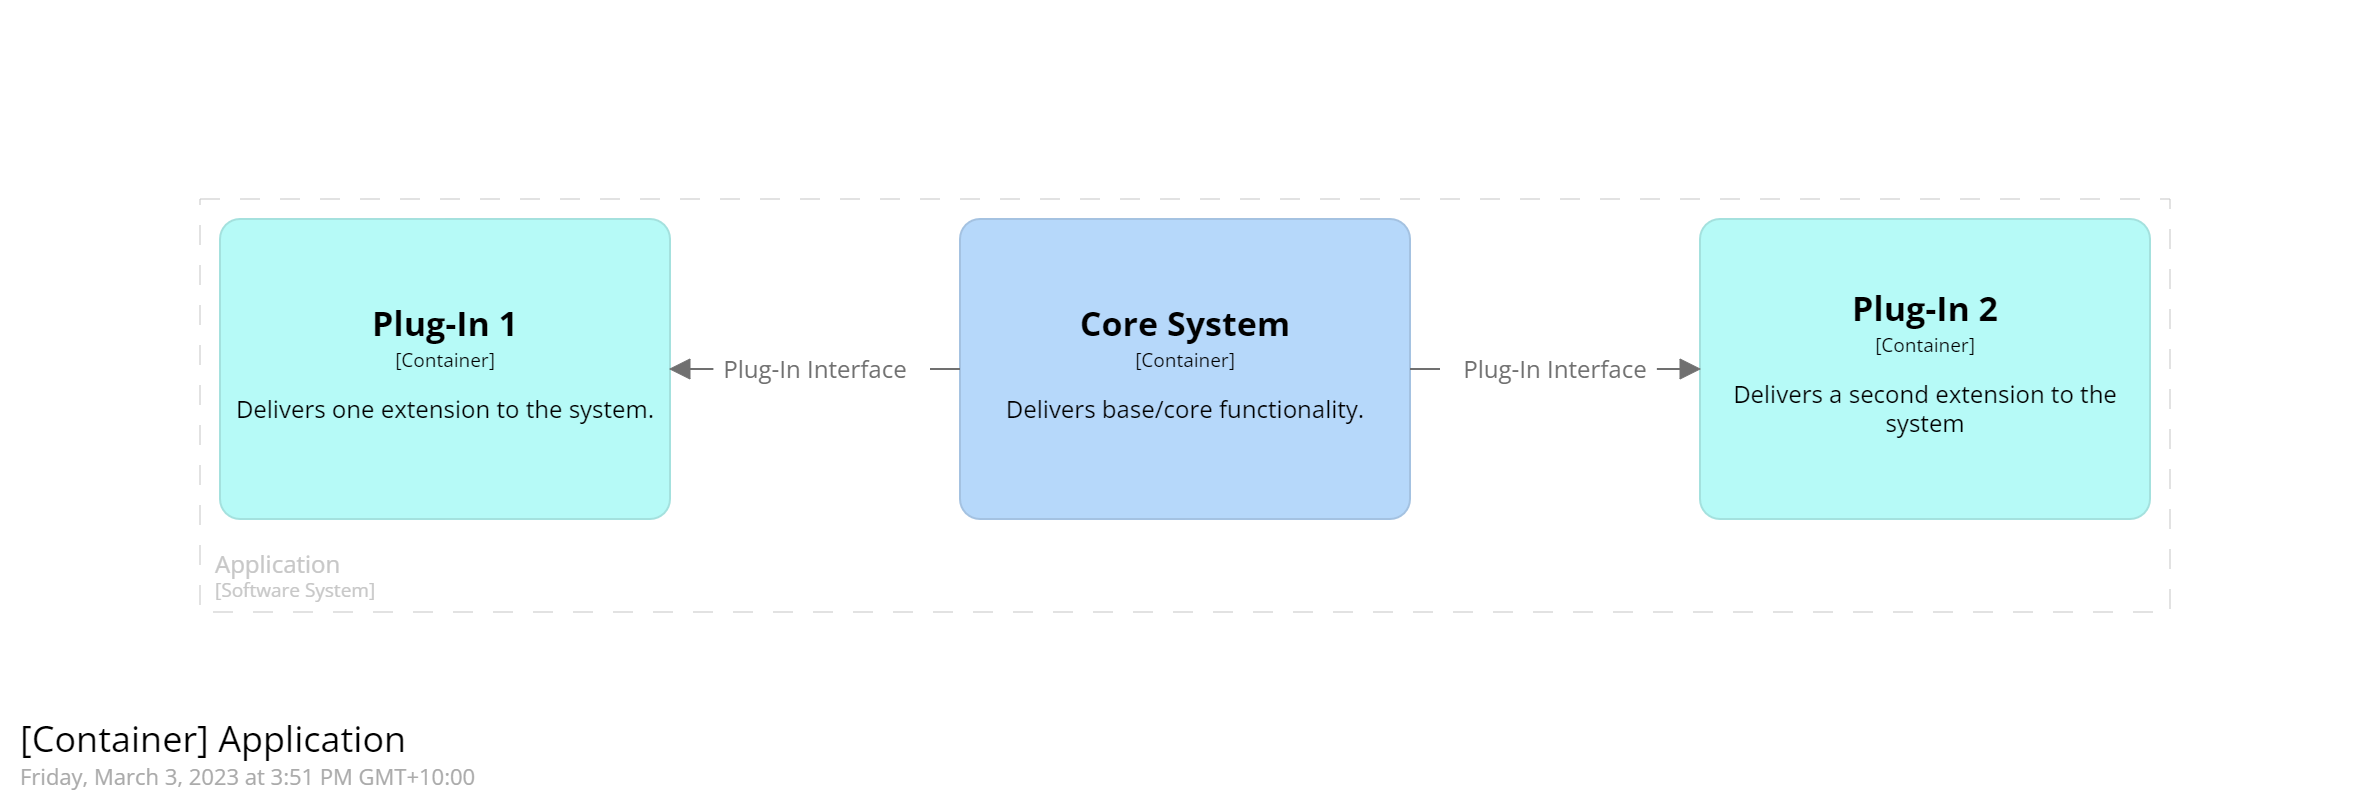
\includegraphics[trim=38 180 22 50,clip,width=\textwidth]{../../notes/microkernel/diagrams/generic-microkernel.png}
\end{frame}
\note[itemize]{
    \item Monolith -- Commonly use method invocation to communicate with plug-ins
    \item Other message passing protocols may be used
}

\definition{Registry}{Tracks which plug-ins are available to the core system and how to access them.}
\note[itemize]{
    \item Monolith -- Registry can be simply plug-in name and reference to delegate object
    \item More detail about communication protocol and data structure required for other message passing approaches
}

\begin{frame}{Loading Plug-ins}
    \vspace{1mm}
    {\huge
    \begin{description}
        \item[Static Loading] when application starts
        \vspace{3mm}
        \item[Dynamic Loading] as needed at run-time
        \vspace{3mm}
        \item[Registry] designed for the selected strategy
    \end{description}
    }
\end{frame}
\note[itemize]{
    \item Dynamic loading requires a plug-in registration and de-registration interface
    \item Could mention that one of the reasons for JARs in Java was to allow dynamic loading of classes
}

\questionanswer{Can you think of a \highlight{microkernel archiecture}?}{Web Browser?}
\note[itemize]{
    \item Eclipse
    \item Operating Systems
    \begin{itemize}
        \item Some Unix variants
        \item Zircon - Google OS kernel
        \item Nintendo Switch OS
    \end{itemize}
    \item Insurance Claims Processing
    \item Payroll
    \item WordPress
}

\definition{Independent Plug-in Principle}{Plug-ins should be independent, with no dependencies on other plug-ins.
The only dependency on the core system is through the plug-in interface.}

\definition{Standard Interface Principle}{There should be a single interface that defines how the core system uses plug-ins.}

\questionanswer{Does a plug-in architecture equate to a microkernel archiecture?}{What about \highlight{IntelliJ}?}
\note{Not really a microkernel, just a large IDE that allows plug-ins.}

\begin{frame}{Plug-ins with Separate Databases}
    \begin{itemize}
        \LARGE\item Plug-ins cannot access core system data
        \begin{itemize}
            \Large\item Core system may pass data to the plug-in
        \end{itemize}
        \LARGE\item Plug-ins may have their own persistent data
    \end{itemize}
    \vspace{1cm}
    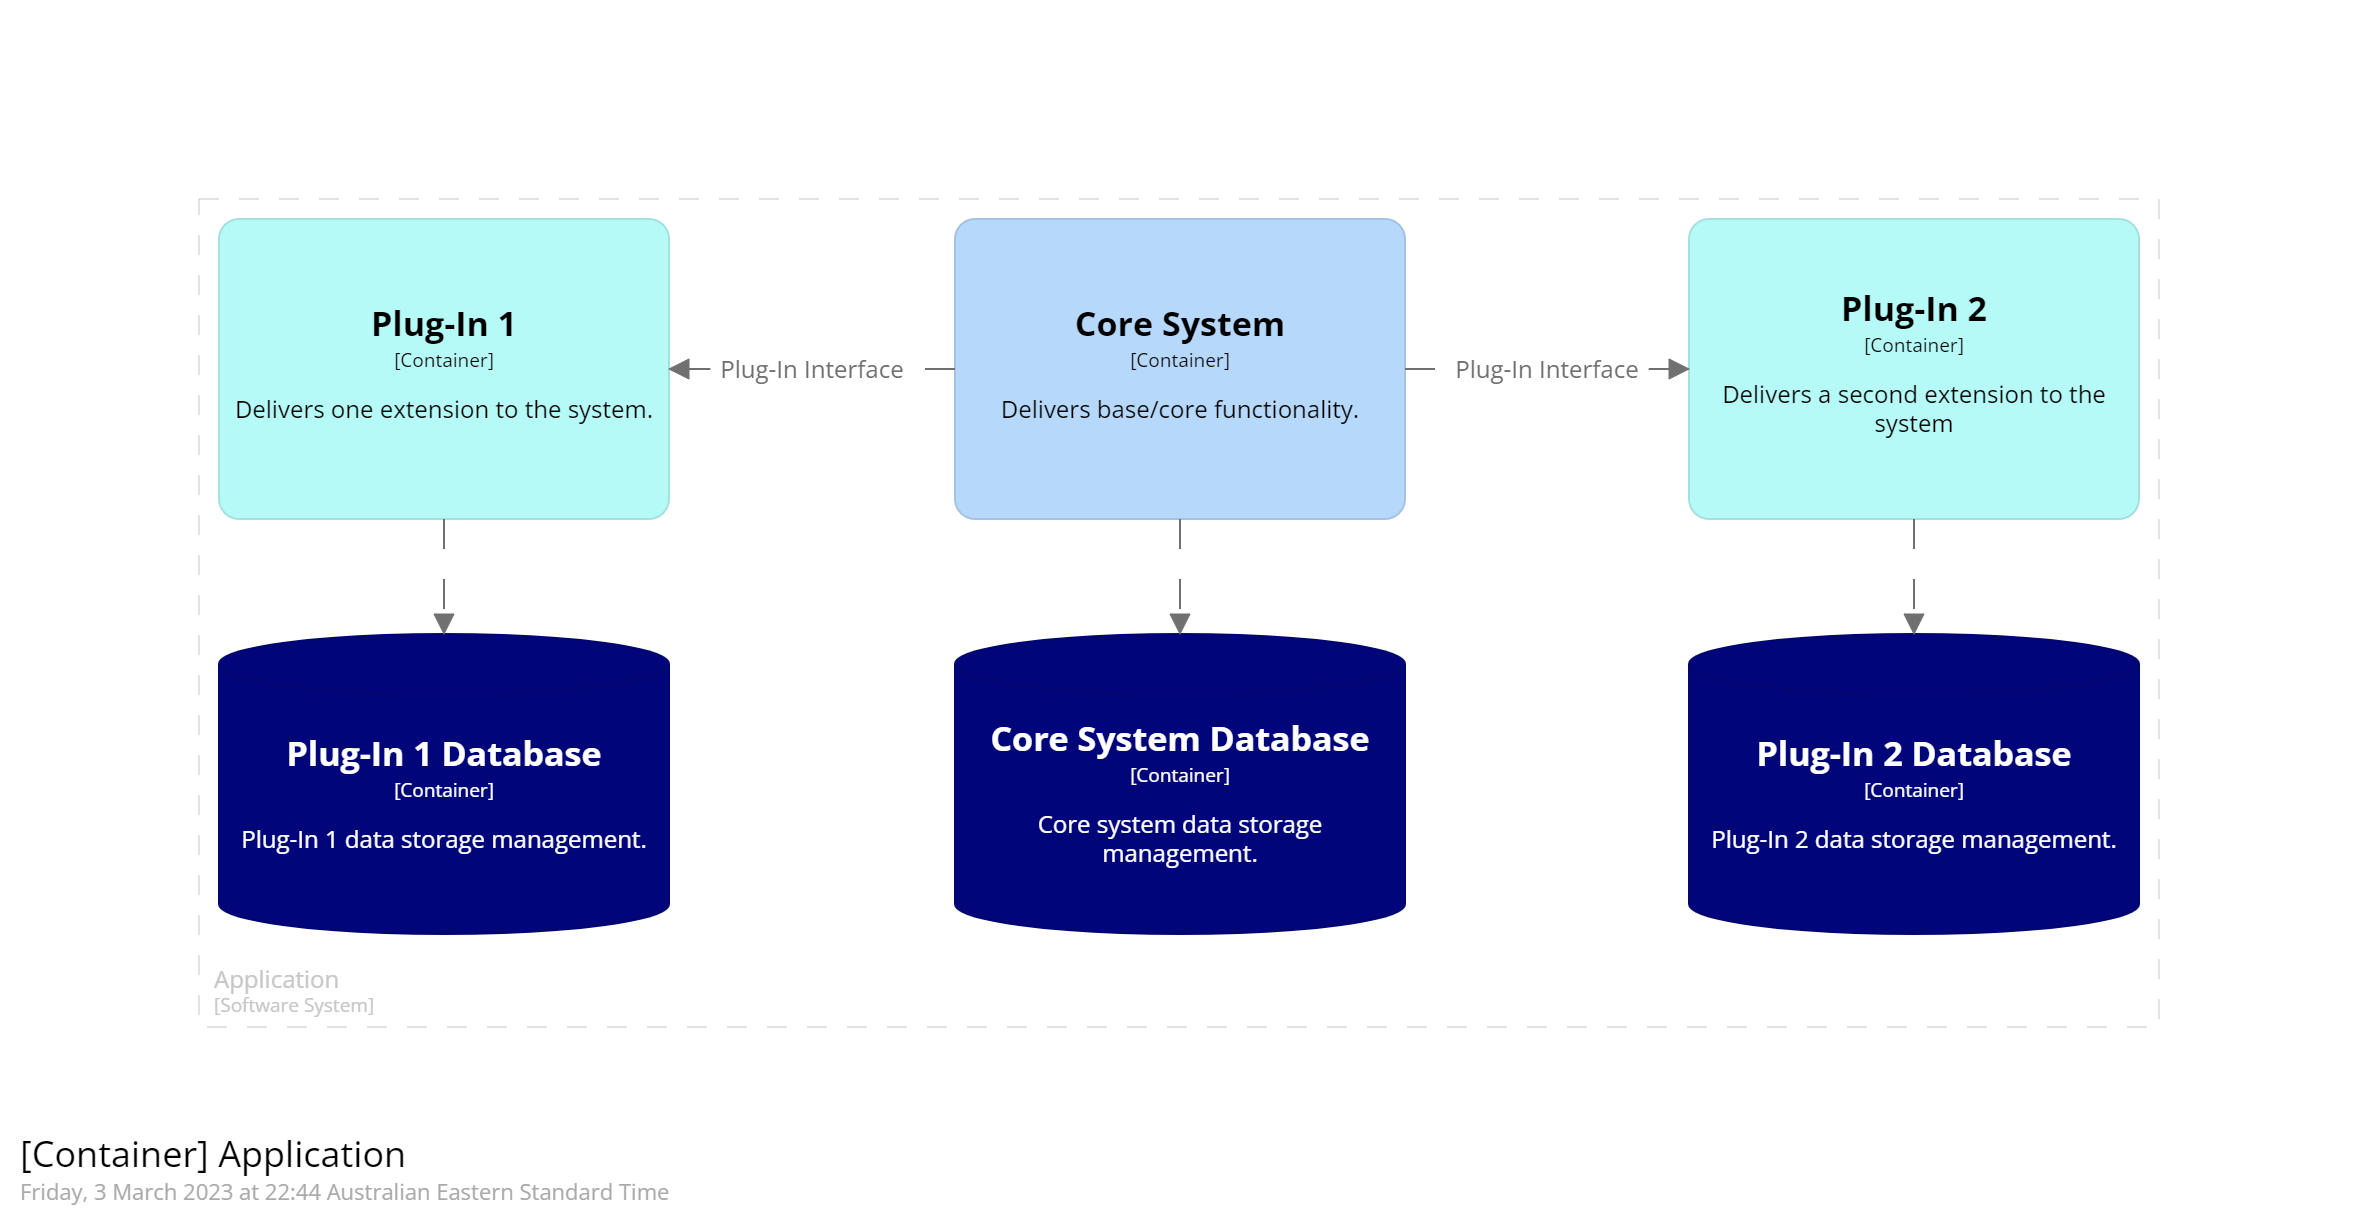
\includegraphics[trim=38 81 24 50,clip,width=\textwidth]{../../notes/microkernel/diagrams/plug-in-databases.png}
\end{frame}

\begin{frame}{Plug-ins as External Services}
    \begin{itemize}
        \LARGE\item Need communication protocol
        \LARGE\item Registry records communication contract
        \begin{itemize}
            \Large\item e.g. URL of the REST endpoint \& data passed to it
        \end{itemize}
    \end{itemize}
    \vspace{1cm}
    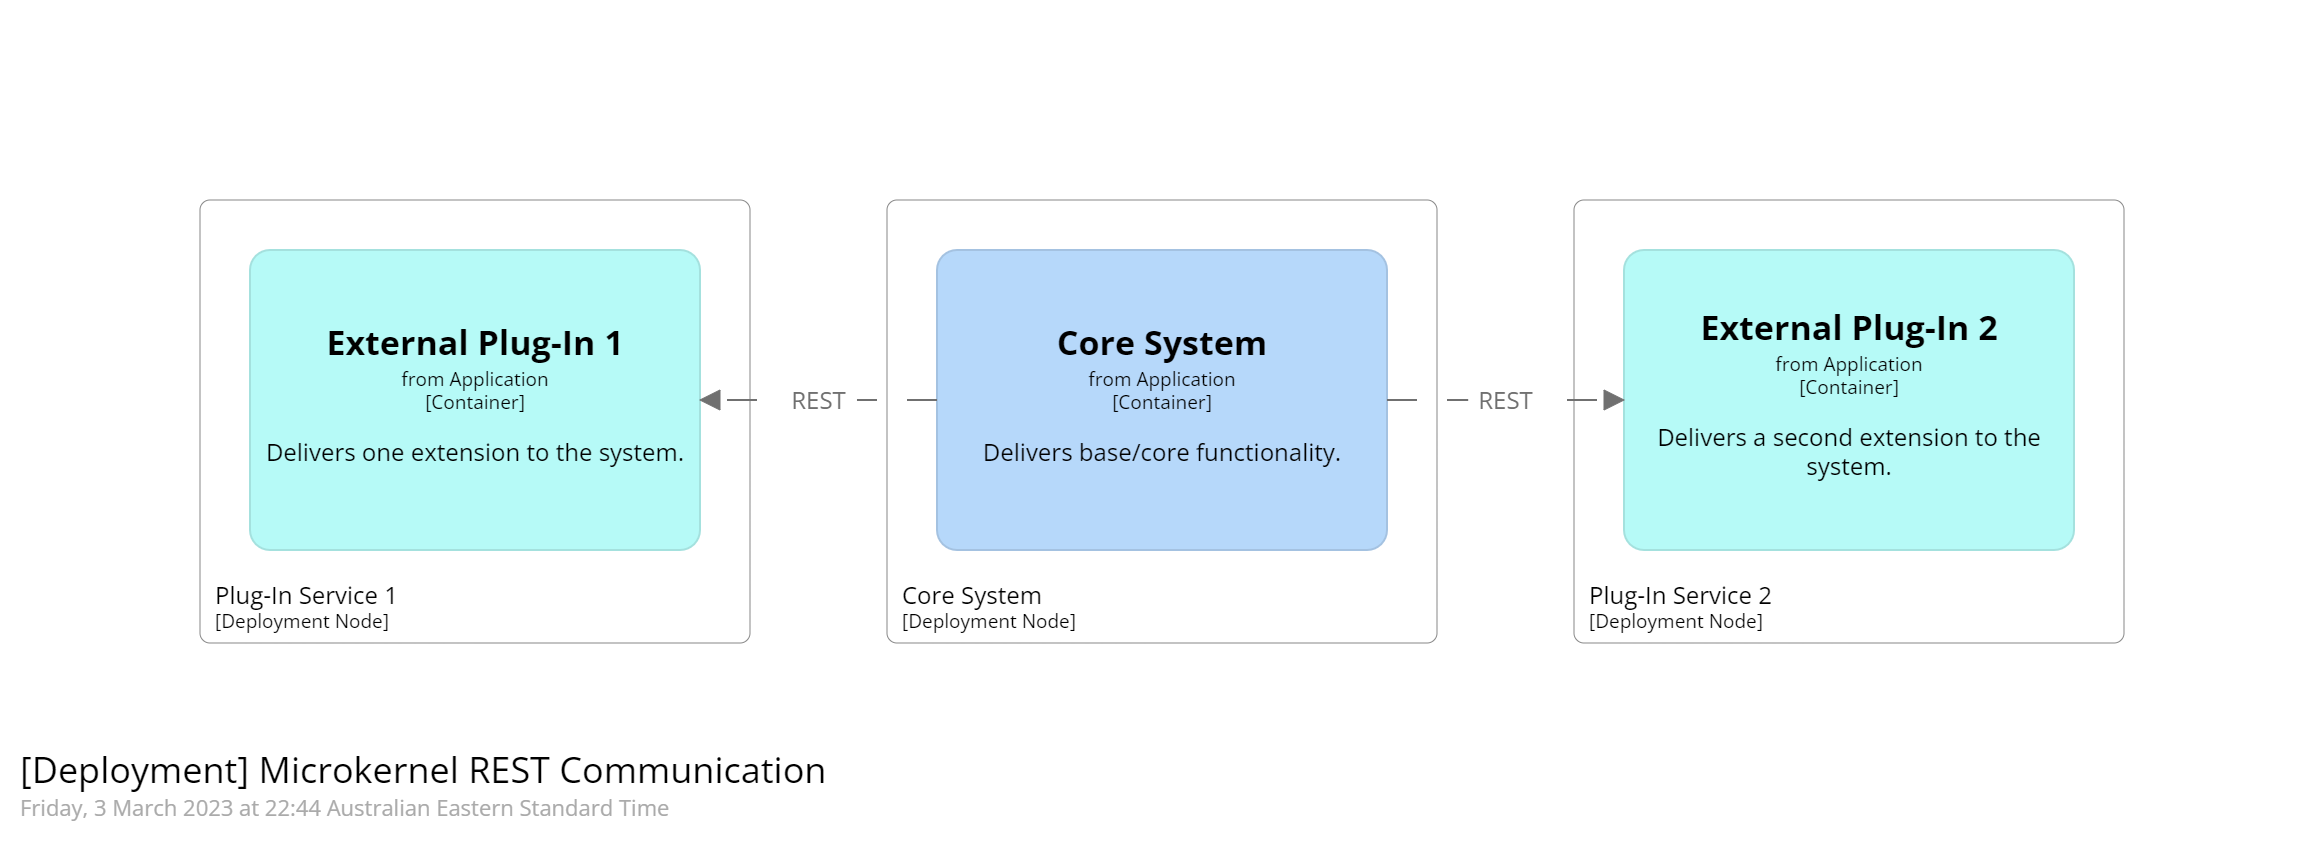
\includegraphics[trim=38 167 19 45,clip,width=\textwidth]{../../notes/microkernel/diagrams/rest-microkernel.png}
\end{frame}
\note[itemize]{
    \item May be deployed on same or separate infrastructure
    \item Allows broad range of communication protocols
}

\begin{frame}{Adapting Non-Conforming Interfaces}
    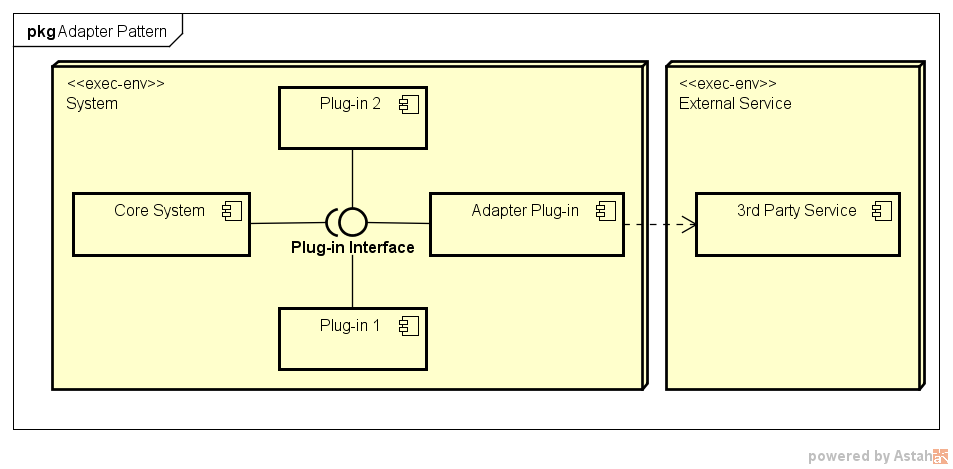
\includegraphics[trim=38 58 20 45,clip,width=\textwidth]{../../notes/microkernel/diagrams/adapter-plug-in.png}
\end{frame}
\note{Introduce \emph{adapter} design pattern as approach to manage 3rd party services as plug-ins}

\begin{frame}
    \vspace{4mm}
    \begin{columns}[t]
    \column<1->{0.5\textwidth}
        \centering
        \LARGE Technical Partitioning
        \begin{figure}
            \centering
            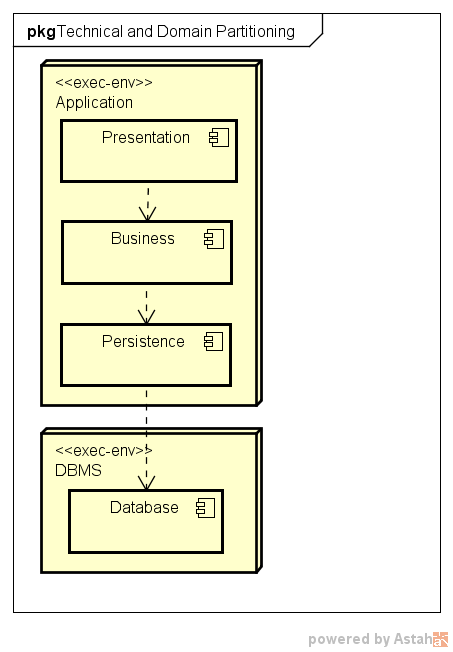
\includegraphics[trim=30 50 142 45,clip,width=0.35\textheight]{diagrams/technical-partitioning.png}
        \end{figure}
    \column<2->{0.5\textwidth}
        \centering
        \LARGE Domain Partitioning
        \begin{figure}
            \centering
            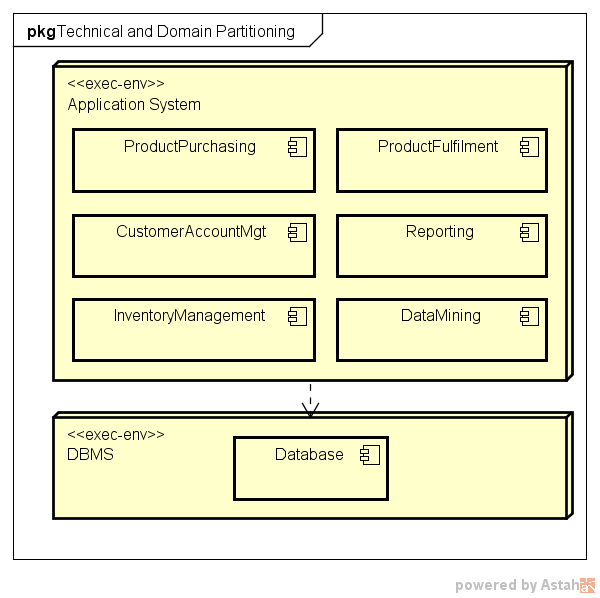
\includegraphics[trim=38 50 19 45,clip,width=\textwidth]{diagrams/domain-partitioning.png}
        \end{figure}
    \end{columns}
\end{frame}
\note[itemize]{
    \item Summarise differences between technical and domain partitioning
    \item Review layered architecture as technical partitioning
    \begin{itemize}
        \item Emphasise it is not the only way to perform technical partitioning
    \end{itemize}
    \item Example of on-line store partitioned into domains
}

\questionanswer{Is the microkernel architecture suited to \highlight{technical} or \highlight{domain} partitioning?}
{Core system can be partitioned either way.}

\begin{frame}{Domain Standard Interfaces}
    \vspace{3mm}
    \centering
    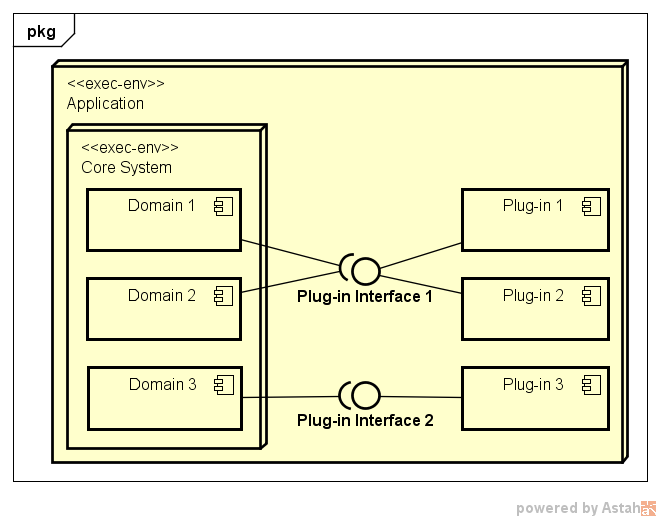
\includegraphics[trim=38 42 23 42,clip,width=1.25\textheight]{../../notes/microkernel/diagrams/domain-microkernel.png}
\end{frame}
\note[itemize]{
    \item Each domain can have its own plug-in interface
    \item Some domains may share a plug-in interface
}

\begin{frame}{Distributed Microkernel}
    \begin{itemize}
        \LARGE\item Partitions in the core system can be distributed
        \begin{itemize}
            \Large\item Technical or domain partitions
            \Large\item Plug-ins could also be distributed
        \end{itemize}
    \end{itemize}
    \vspace{3mm}
    \centering
    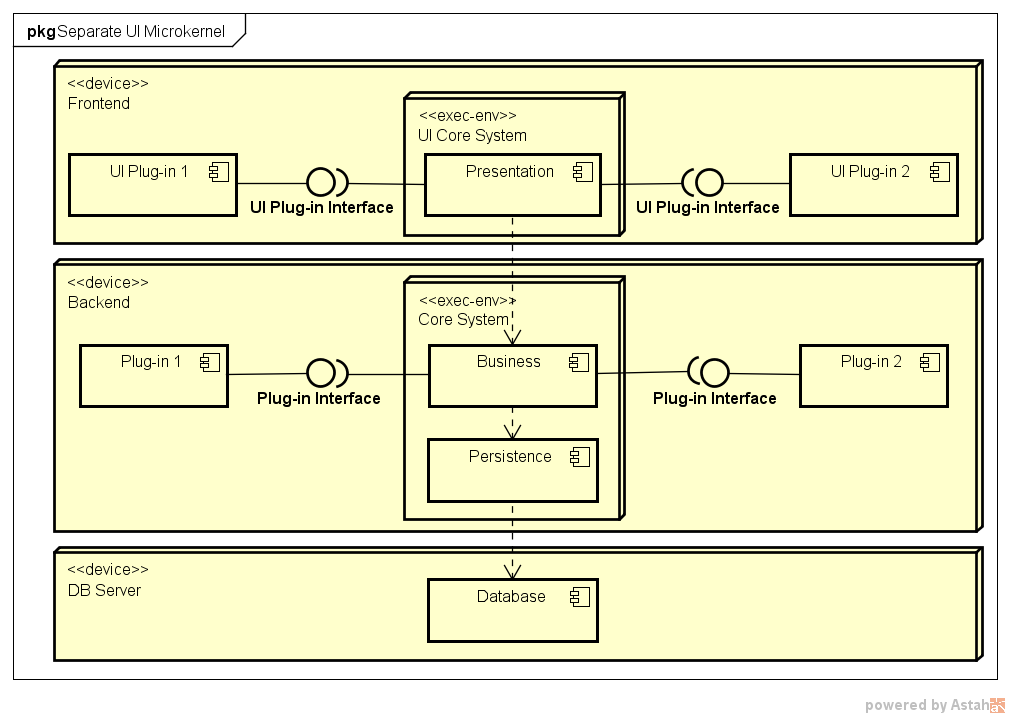
\includegraphics[trim=39 138 19 43,clip,width=0.7\textwidth]{../../notes/microkernel/diagrams/separate-ui-microkernel.png}
\end{frame}
\note{Comment on additional complexity}

\begin{frame}{Pros \& Cons}
    \vspace{1mm}
    {\huge
    \begin{description}
        \item[Simplicity] Core system \& Plug-in interface \tabto{15em}
\includegraphics[width=10mm]{../../shared/images/thumbs-up.png}
        \item[Extensibility] Plug-ins \tabto{15em}
\includegraphics[width=10mm]{../../shared/images/thumbs-up.png}
        \item[Interoperability] Plug-ins \tabto{15em}
\includegraphics[width=10mm]{../../shared/images/thumbs-up.png}
        \item[Scalability] \tabto{15em}
\includegraphics[trim=22 19 22 15,clip,width=10mm]{../../shared/images/thumbs-down.png}
        \item[Reliability] \tabto{15em}
\includegraphics[trim=22 19 22 15,clip,width=10mm]{../../shared/images/thumbs-down.png}
    \end{description}
    }
\end{frame}

\end{document}